This section describes the exploration of the software/hardware co-design space.
The software side includes partitioning the program, determining the number of threads and the specific source-level optimisations.
The hardware side is about finding out the best core composition that maximizes performance for a given partitioning.

\subsection{Thread Partitioning}

This section first starts with analyzing the impact of thread partitioning on performance.
In this section, the term optimal number of threads defines the number of threads which results in the best performance for any given benchmark.
Thread partitioning is about deciding how many threads to create and how to partition StreamIt filters into these threads.

To simplify this study, the default streaming partitioner is used to decide on how to allocate filters to threads which is based on simulated annealing~\cite{simulatedAnnealing1983}.
On the hardware side, two scenarios are considered: the ``without composition scenario'' where there is exactly one core per thread and the ``with composition scenario'' where each thread receives between 1 and 15 cores.
Figure~\ref{fig:threadtrend} shows how performance varies under both scenarios as a function of the number of threads.
In this figure, the ``with composition scenario`` uses points from the sample space that result in the fastest execution time for a given number of threads.
Regardless of how cores are composed it can be observed that curves for a benchmark follow the same trend.
As can be seen in Figure~\ref{fig:threadtrend}, the optimal number of threads using core composition is very similar to the scenario without composition as both curves follow the same performance trends.
This is due to the fact that StreamIt is oriented towards task-level parallelism and thus, multithreading will be a natural fit for performance improvements whilst core-composition may have less of an effect overall.
As Figure~\ref{fig:threadtrend} shows that the performance trends for both with and without composition are similar when it comes to thread counts, this  means that the optimal number of threads for a benchmark can be estimated independently from the hardware composition.
The system can therefore proceed in two stages: first determine the optimal number of threads and then decide on a core composition.

Figure~\ref{fig:threadtrend} also shows that the performance of most benchmarks starts to deteriorate passed a certain number of threads making it critical to not over-allocate threads.
This number of threads varies between benchmarks, thus it motivates the use of machine learning to decide the optimal number of threads to use.
Finally it is important to observe that executions without compositions always perform worse.
This demonstrates that composing cores is essential to obtain the best performance from a workload.


\subsection{Core Composition}

\begin{figure}[t]
  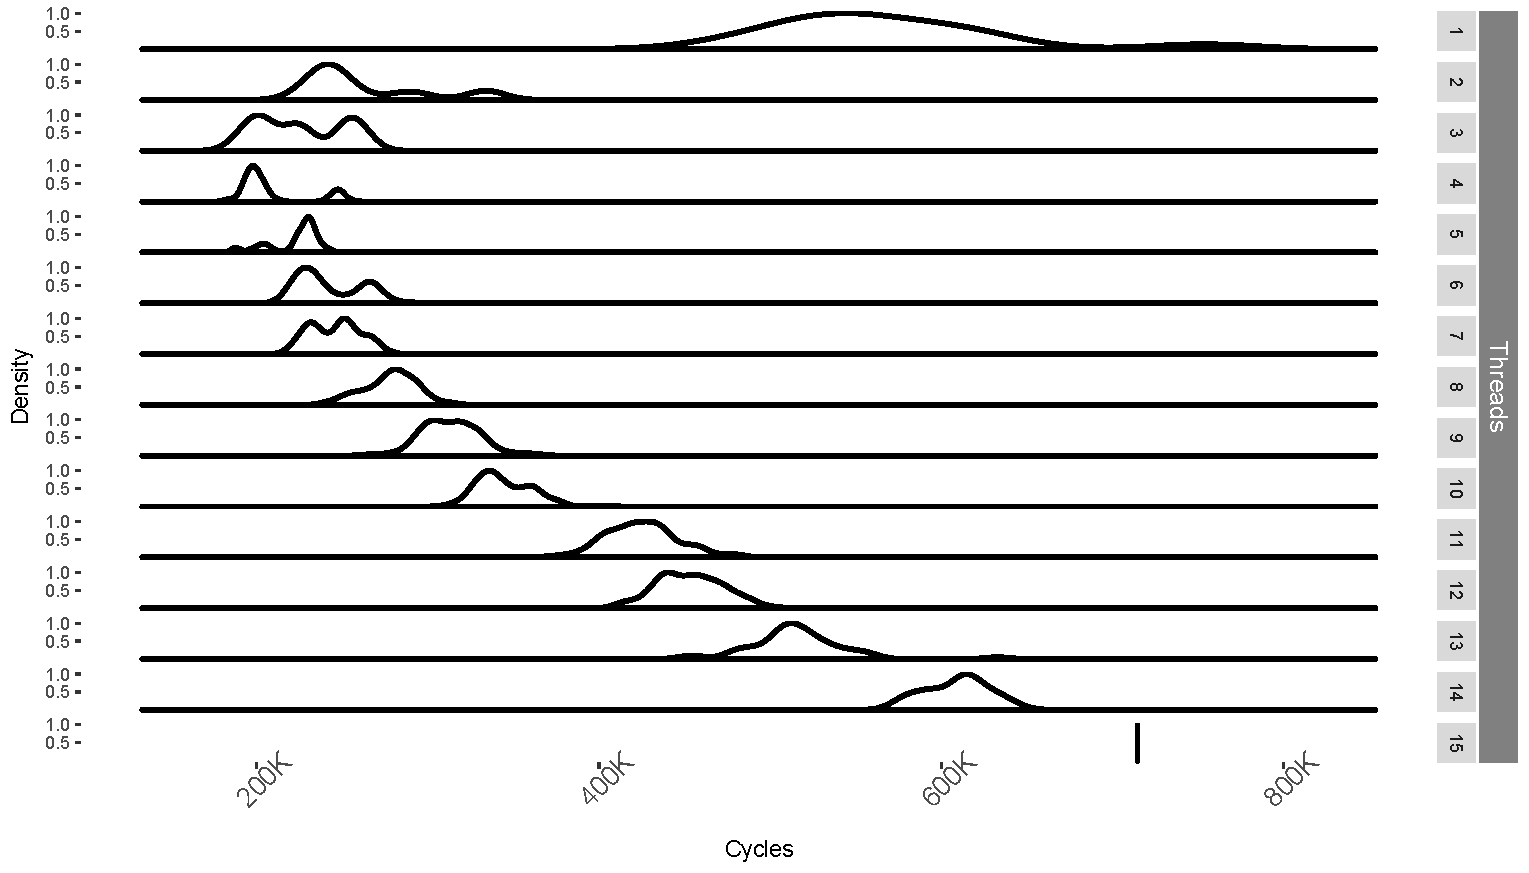
\includegraphics[width=1\textwidth]{streamit-paper/graphics/filterbank_tot.pdf}
  \caption{Distribution of FilterBank performance when modifying the amount of threads and compositions.}\label{fig:fbtotal}
\end{figure}

Using core composition, the processor fuses a number of cores and associates them to a thread to increase single threaded performance.
Whilst this flexibility is advantageous, choosing the right amount of cores for a given thread is difficult due to the large number of possible configurations~\cite{gulati2008multitaskingdmc}.

Figure~\ref{fig:fbtotal} shows how threading and core-compositions affect performance for the \bench{FilterBank} benchmark.
The curves represent the density distribution for different core compositions as a function of the number of threads.
The right hand side Y-axis represents the number of threads present in the current version of the benchmark whilst the left Y-Axis represents the density normalized by the total number of points in the design space.
For each of the threaded versions the benchmark runs using 100 different core-compositions.
The density curve for thread 15 is a single point as there exists only a single composition, so a line is drawn to represent where that point lies.

The width of each of the curves represents the influence of composition on the \bench{FilterBank}'s performance for a given number of threads.
For this benchmark, the impact of having core-composition enabled often leads to a 1.5x speedup compared to running only in multi-threaded mode; this can be seen for 1 to 4 threads.
Interestingly, as more threads are used, performance worsens, echoing the results shown in the previous section.
This is due to the fact that when the number of threads is increased, synchonization between threads will increase whilst the potential number of corse which can be fused decreases.
In the case where the application does not feature highly parallel tasks, de-prioritising core compositions can negatively impact performance.
This signifies that for the benchmark \bench{FilterBank}, it is more important to fuse cores with a small amount of threads rather than add more and more threads to the application.


\begin{figure}[t]
  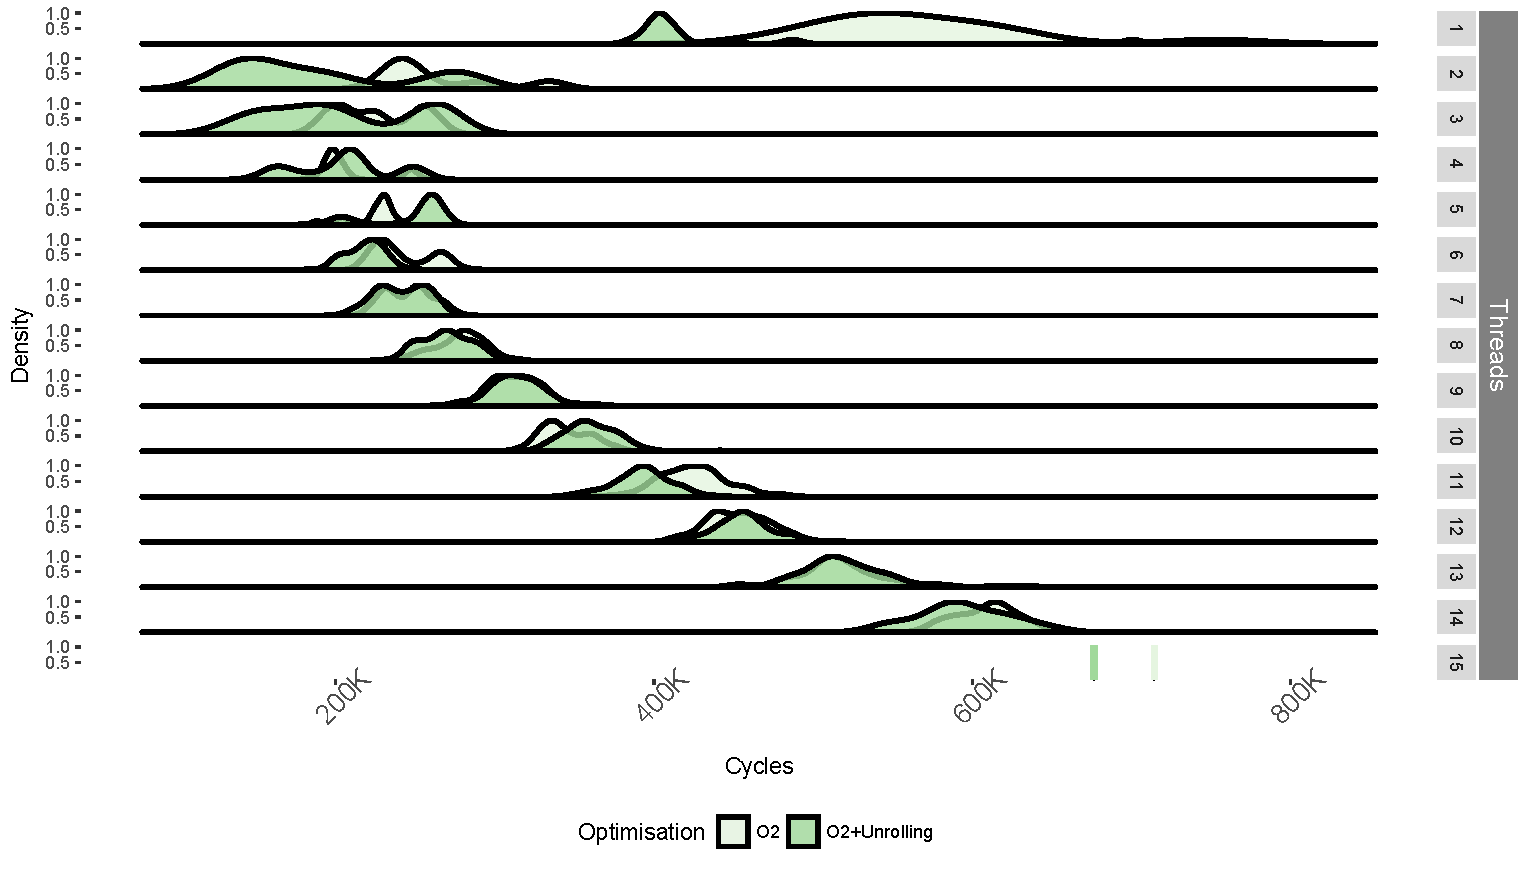
\includegraphics[width=1\textwidth]{streamit-paper/graphics/filterbank_unroll.pdf}
  \caption{Distribution of FilterBank performance when modifying the amount of threads, composition and unrolling factor.}\label{fig:fbunroll}
\end{figure}


\subsection{Impact of Loop Transformation}
As seen in Chapter~\ref{chp:Background}, composing cores exploits block-level parallelism by running multiple EDGE blocks on a logical core.
As physical cores in a logical core must communicate to submit block address predictions, and commit information to each other, having a small number of blocks will reduce the communication overhead.
Since physical cores can fetch more than a single block when the blocks are made of a small number of instructions, finding methods to increase the average size of the blocks can lead to reduced overhead.
One method of increasing the size of the blocks is through loop unrolling.
This section therefore analyses the impact of loop unrolling on the StreamIt benchmarks.

In this Chapter, unrolling is done at the source level via a flag passed to the StreamIt source-to-source compiler.
Given a number of times the loops must be unrolled, the StreamIt source-to-source compiler will generate the multi-threaded C++ code with the loops manually unrolled.
Figure~\ref{fig:fbunroll} presents an example of how loop unrolling affects performance on the \bench{FilterBank} benchmark.
The graph presents the same information as Figure~\ref{fig:fbtotal} but comparing .
Figure~\ref{fig:fbunroll} shows that unrolling loops for \bench{FilterBank} can improve performance by up to 1.42x compared to the fastest non-unrolled version.
Another observation is that the best execution times for each of the threaded versions when unrolling does not follow the same trend seen in Figure~\ref{fig:threadtrend}.
The leftmost curve performance peaks at two threads whereas the rightmost peaks at 3 compared to 4 in the non-unrolled version.

\begin{figure}[t]
  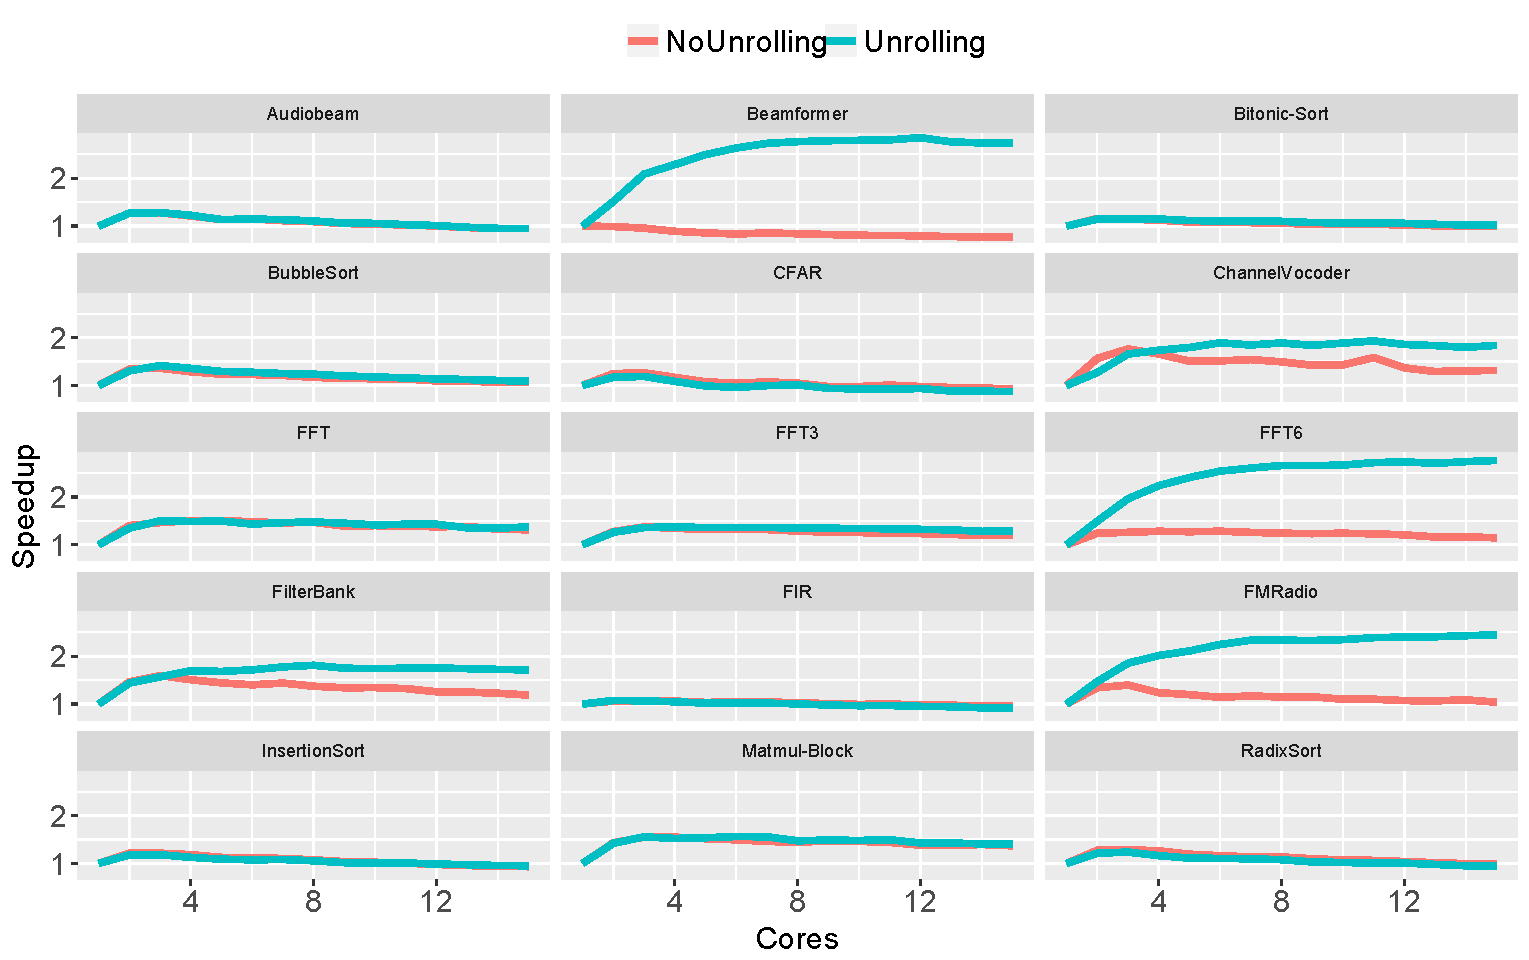
\includegraphics[width=1\textwidth]{streamit-paper/graphics/unrolling_vs_no_single_core.pdf}
  \caption{How unrolling affects how much performance can be obtained via core-composition on the single-threaded versions of each benchmarks.}\label{fig:unroll_summary}
\end{figure}

Figure~\ref{fig:unroll_summary} goes into more details on how unrolling affects the amount of speedup obtained by running each of the StreamIt benchmarks on a single thread using different number of cores in the composition.
In this figure, the X axis represents the number of cores in the composition, ranging from single core to 15.
The Y axis compares the execution time in number of cycles for the benchmark using a single core vs a given core-composition.
The colours of the lines represent with and without unrolling.
As can be seen, for the set of benchmarks used throughout this chapter, five benchmarks benefit from unrolling.
These benchmarks are \bench{Beamformer}, \bench{ChannelVocoder}, \bench{FFT6}, \bench{FilterBank} and \bench{FMRadio}. 

\begin{figure}[t]
  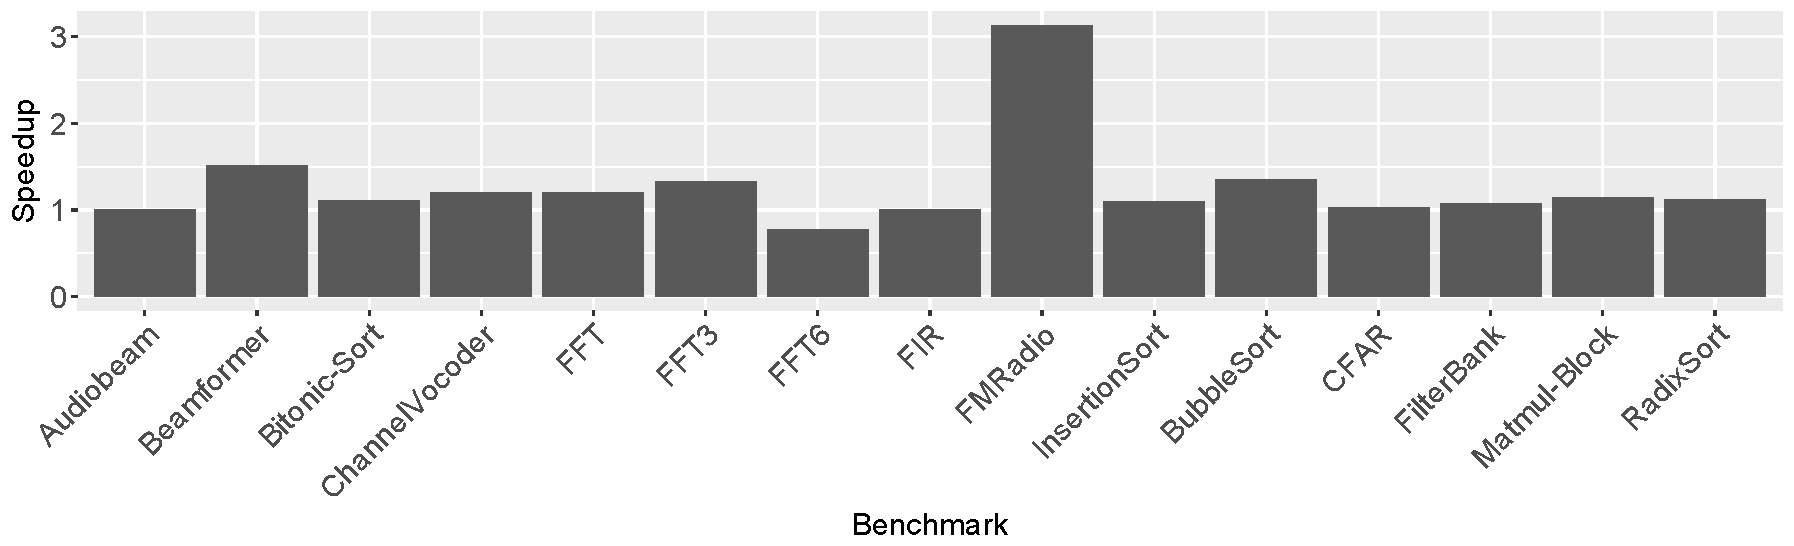
\includegraphics[width=1\textwidth]{streamit-paper/graphics/unroll_speed_bars.pdf}
  \caption{Speedup obtained .}\label{fig:unroll_bars}
\end{figure}
Figure~\ref{fig:unroll_bars} complements Figure~\ref{fig:unroll_summary} by showing the speedup obtained by unrolling loops when executing the benchmark on a single core.
On average, the information shown in Figure~\ref{fig:unroll_bars} coincides with the data shown in Figure~\ref{fig:unroll_summary}: benchmarks that don't scale also see no difference in performance when loop unrolling is called.
For the benchmarks that do not scale with unrolling; this is most certainly due to the for loops containing conditional statements which may keep the blocks size small.
When a loop that holds multiple conditional statements is unrolled, conditional statements may not be fused into a single block; thus the block size does not change.
Benchmark \bench{FMRadio} sees a 3x improvement compared to the non-unrolled version, this is due to the fact that all the loops are fully unrolled, reducing the total number of instructions required to execute the task.
For the \bench{FFT6} benchmark, unrolling loops will actually cause the single-core version to be slower than its not unrolled version.
%I think this is due to a refreshing performance thing
This is due to the fact that the increased size of the blocks increases the latency of fetching larger blocks.
Whilst it may be slower on a single core, as seen in Figure~\ref{fig:unroll_bars}, having a core-composition running the thread will still result in faster execution that without loop-unrolling.

Figure~\ref{fig:unroll_size} shows the influence of loop unrolling on the average size of an EDGE block for each of the benchmarks.
The size represents the number of instructions exected in each of the EDGE blocks.
As can be seen, the data for \bench{Beamformer} and \bench{FFT6} in Figure~\ref{fig:unroll_size} corroborate with the idea that larger block sizes will result in better performance when fusing cores.
However whilst benchmarks \bench{ChannelVocoder}, \bench{FilterBank} and \bench{FMRadio} also see an increase in blocksize, it is not as important and averages out at a 1.22x increase.
%Be clearer here.
That said, even a small amount of increase can help improve the scalability of core-composition.

\begin{figure}[t]
  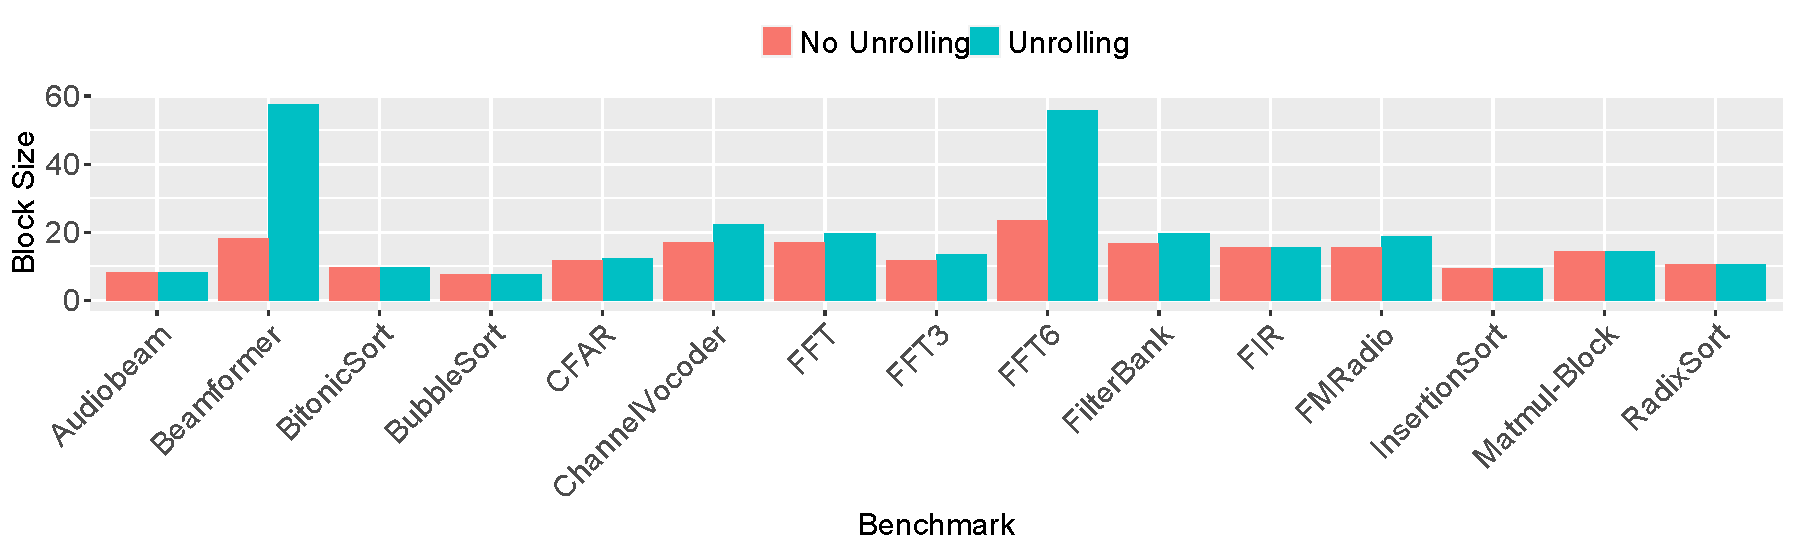
\includegraphics[width=1\textwidth]{streamit-paper/graphics/unrolling_size.pdf}
  \caption{Average size (in instructions) of blocks executed with and without unrolling for each benchmark .}\label{fig:unroll_size}
\end{figure}

Overall, this section has shown that loop unrolling can improve performance by increasing the size of blocks for the benchmarks which helps improve the efficiency of core-compositions.

\subsection{Co-Design Space Best Results}


This section  presents the results of the entire co-design space exploration.
Figure~\ref{fig:overviewhist} characterizes how much of a performance increase, over a baseline of a single-core single-thread with O2 optimisations, can be obtained with and without unrolling.
For each benchmark, the \textit{THREAD} bar represents the maximal speedup obtained by dividing the program into threads without fusing cores.
The \textit{CORE} bar represents the best speedup when the benchmark is executed in a single thread and fuse cores.
\textit{BOTH} represents the best speedup obtained for each benchmark using a combination of \textit{THREAD} and \textit{CORE}.
Finally, for each benchmark, the results are obtained for both an unrolled and not unrolled version to compare how the compiler optimisation affects performance.
Figure~\ref{fig:overviewhist} shows that when loops are not unrolled, composing cores will not greatly improve performance.
This is due to the fact that the amount of ILP found in filters without the unrolling is too little for there to be any benefit of composing cores.

In the scenario where there are no specific optimisations for composition, multithreading will be the main source of performance.
This can be seen when studying the geometric mean,without unrolling.
Finding the optimal number of threads gives a speedup of 1.92 compared to 1.33 when using only core composition, which is an improvement of 44\%.
This changes when taking unrolling into account as the core compositions can be used more efficiently.
In this case, the speedup obtained from only composing cores is only 13\% worse than using only threads.
For the \bench{FMRadio} benchmark, unrolling makes using only core-composition better than only using threads.
This information corroberates with the data seen in Figure~\ref{fig:unrolling_vs_no_single_core}; it presents a unique case where the effect of core composition is important enough to change the dominant performance enhancer.
%Thus loop unrolling demonstrates that the StreamIt programs must be modified to take advantage of the core composition.

Overall the results demonstrate that multi-threading is the prevalent leader of performance, even with unrolling turned on.
This is natural as StreamIt applications are naturally geared towards TLP as most programs have at least one SplitJoin as seen in the Table~\ref{tab:splitjoin} which gives the number of split-joins per benchmark.
Benchmarks with SplitJoins will naturally benefit from splitting the program into threads~\cite{thiesStreamit2010}.
%Make sure this is 100% true but as far as I remember this is the case
Those that do not feature SplitJoins can still be parallelised by splitting a Pipeline into multiple parts.
For example, benchmark \bench{FIR} features no SplitJoins, yet splitting the Pipeline in 2 will result in a 1.40x speedup.
However, it is important to note that whilst finding the optimal thread mapping may result in higher performance improvements than finding the optimal composition for a single thread, the best performance is always obtained through a combination of both optimizations.
For cases such as \bench{BeamFormer} the optimal pairing results in a 1.8x speedup compared to simply finding the best multit-threaded version.
On average, the optimal combination leads to a 1.5x performance increase compared to only multithreading.

\begin{landscape}
\begin{figure}\hspace{-1em}
    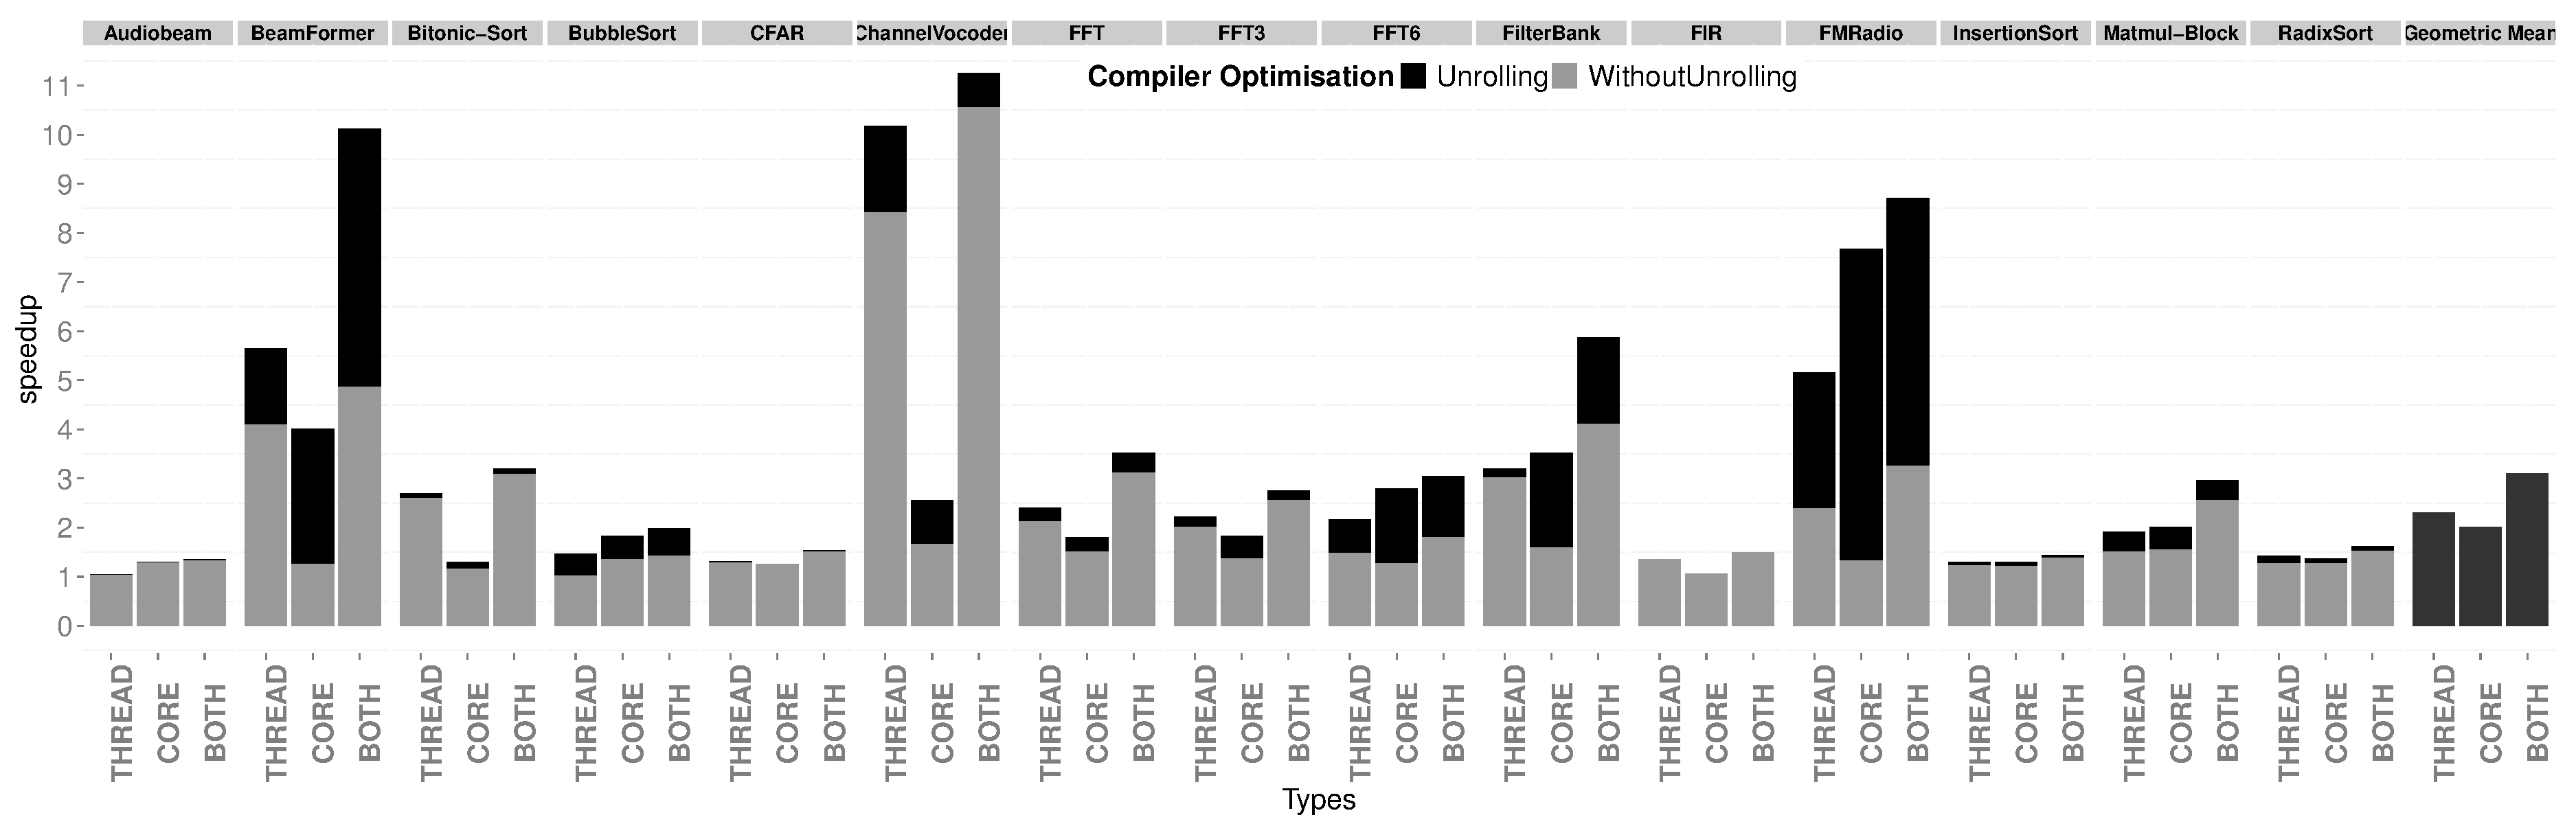
\includegraphics[width=1\linewidth,keepaspectratio]{streamit-paper/graphics/threadcompbench.pdf}
    \caption{Speedup obtained by choosing best core composition, best
      thread number and the combination of both optimisations. The baseline for the speedup measurement is single core, single thread execution using O2 compiler optimisations. Higher
      is better.}\label{fig:overviewhist}
\end{figure}
\end{landscape}
\subsection{Summary}
This section demonstrated that each parameter has a large effect on the performance of the workload.
Regardless of using core composition or not, there exists for each benchmark an optimal number of threads.
Unrolling is effective at exposing more opportunities for composition due to increased ILP but there is a balance to strike between extracting ILP and TLP.
Figure~\ref{fig:overviewhist} shows there is a 3x benefit (overall) by automating the partitioning of both the software (threads) and hardware (cores).

